\documentclass[conference]{IEEEtran}
\IEEEoverridecommandlockouts

\usepackage{cite}
\usepackage{amsmath,amssymb}
\usepackage{graphicx}
\usepackage{booktabs}
\usepackage{multirow}
\usepackage{xcolor}
\usepackage{tikz}
\usetikzlibrary{arrows.meta,positioning,fit,calc}
\usepackage{fontspec}
\newfontfamily\telugufont{NotoSansTelugu-Regular.ttf}[Path=./fonts/, Script=Telugu]
\usepackage[hidelinks]{hyperref}

% Values that come from the full training run are shown in red until they are filled in.
\newcommand{\pending}[1]{\textcolor{red}{#1}}

\begin{document}

\title{TruthLens AI: An Explainable Multilingual Multimodal System for Fake News and AI-Generated Image Detection with Contradiction-Aware Claim Verification}

\author{
\IEEEauthorblockN{K. Srivalli}
\IEEEauthorblockA{\textit{Dept. of IT, SRGEC}\\
Gudlavalleru, India\\
\phantom{email@srgec.ac.in}}
\and
\IEEEauthorblockN{I. Bhargavi}
\IEEEauthorblockA{\textit{Dept. of IT, SRGEC}\\
Gudlavalleru, India\\
\phantom{email@srgec.ac.in}}
\and
\IEEEauthorblockN{I. Teja Sai}
\IEEEauthorblockA{\textit{Dept. of IT, SRGEC}\\
Gudlavalleru, India\\
\phantom{email@srgec.ac.in}}
\and
\IEEEauthorblockN{K. Lakshmi}
\IEEEauthorblockA{\textit{Dept. of IT, SRGEC}\\
Gudlavalleru, India\\
\phantom{email@srgec.ac.in}}
\and
\IEEEauthorblockN{Y. K. Viswanadham}
\IEEEauthorblockA{\textit{Assoc. Prof., Dept. of IT, SRGEC}\\
Gudlavalleru, India\\
\phantom{email@srgec.ac.in}}
}

\maketitle

\begin{abstract}
Most fake news detectors return a single label for a whole article and say nothing about which statements are false or why. They also tend to support only English and only text. We present TruthLens AI, a system that checks English and Telugu news text and also flags images that are AI-generated. Text is classified with a fine-tuned DeBERTa-v3-large model for English and IndicBERT v2 for Telugu. Images are classified by a linear probe on CLIP ViT-L/14 features. LIME marks the words behind each text verdict, and Grad-CAM marks the image regions behind each image verdict. The main extension is claim-level verification: the system splits an article into check-worthy claims, retrieves evidence with BGE-M3 embeddings and a FAISS index, and labels each claim Support, Contradiction or Unknown with a natural language inference (NLI) model. The claim results are combined into a credibility score and then fused with the classifier output. On the cleaned WELFake test set, DeBERTa-v3-large reaches 99.7\% accuracy against 98.8\% for a BERT-base baseline. The Telugu model reaches 93.1\% and the image detector 93.7\%. With gold evidence, contradiction-aware verification reaches 84.6\% accuracy (macro-F1 0.847) on FEVER and 50.9\% (macro-F1 0.467) on the harder, real-world Climate-FEVER set, while a similarity-only baseline reaches 40.0\% and 34.0\% and cannot detect a single refuted claim. We also report a bias check showing that a TF-IDF model scores 96.2\% on WELFake, which limits what high accuracy on that dataset can prove.
\end{abstract}

\begin{IEEEkeywords}
fake news detection, claim verification, natural language inference, explainable AI, Telugu, AI-generated image detection, DeBERTa, CLIP
\end{IEEEkeywords}

\section{Introduction}

False stories reach people faster and further than true ones. In a study of about 126,000 stories shared on Twitter between 2006 and 2017, false news reached 1,500 people roughly six times faster than true news \cite{vosoughi2018spread}. In Andhra Pradesh and Telangana much of this content circulates in Telugu on WhatsApp, often next to an image, and the image is now as likely to be generated by a diffusion model as photographed.

Automatic detectors exist, but three gaps make them hard to use for this audience. First, most are trained and tested on English only. Second, they treat text and images separately. Third, and most important for a reader who wants to decide whether to forward a message, they output one label for a whole article. A label of ``Fake, 91\%'' does not tell the reader that the article's date is right but its central number is invented.

TruthLens AI is built around that third gap. Besides a whole-article classifier, it extracts individual claims, finds evidence for each, and uses an NLI model to decide whether the evidence supports or contradicts the claim. A claim that matches the evidence but is negated by it is reported as contradicted, not as ``related'', which is what a similarity search alone would report. Our contributions are:

\begin{itemize}
\item A working system that checks English and Telugu text and images, runs on an ordinary laptop with one command, and processes single items or batches through a web interface.
\item A contradiction-aware verification stage with an explicit decision rule (Section~\ref{sec:verify}), evaluated on FEVER, Climate-FEVER and a curated Indian-news claim set, and compared with a similarity-only baseline.
\item A Telugu training set built by translating both classes of WELFake with NLLB-200, after showing that an existing Telugu dataset can be separated by writing style alone.
\item Explanations at the level a reader can act on: highlighted words (LIME), highlighted image regions (Grad-CAM), and per-claim evidence with its source.
\end{itemize}

\section{Related Work}

\subsection{Text-based fake news detection}
Early work used hand-built features such as word counts, punctuation and source metadata \cite{shu2017fake}. Benchmarks such as LIAR \cite{wang2017liar} and WELFake \cite{verma2021welfake} made supervised comparison possible; WELFake merges four earlier corpora into 72,134 articles. Fine-tuned transformers now dominate. FakeBERT combined BERT \cite{devlin2019bert} with convolutional layers \cite{kaliyar2021fakebert}. DeBERTa improves on BERT by encoding content and position separately \cite{he2021deberta}, and DeBERTa-v3 adds ELECTRA-style replaced-token pre-training \cite{he2023debertav3}. We use DeBERTa-v3-large as the English classifier and BERT-base as the baseline.

\subsection{Indian-language resources}
Indian languages have far fewer labelled fake news datasets. BanFakeNews provides about 50,000 Bangla articles \cite{hossain2020banfakenews}. For Telugu, a public dataset is available on Zenodo \cite{telugu2024zenodo}, which we examine in Section~\ref{sec:data}. Multilingual encoders trained on Indian text, such as IndicBERT \cite{kakwani2020indicnlp} and IndicBERT v2, which covers 23 Indian languages \cite{doddapaneni2023indicbertv2}, make Telugu classification practical. NLLB-200 translates between 200 languages, including English and Telugu \cite{nllb2022}.

\subsection{AI-generated image detection}
Wang et al. showed that a ResNet trained on one GAN's images generalises to other GANs \cite{wang2020cnndetect}, but such detectors transfer poorly to diffusion models \cite{corvi2023diffusion}. Ojha et al. found that a linear classifier on frozen CLIP \cite{radford2021clip} features generalises better across generators than a fully trained network \cite{ojha2023universal}. We follow that approach. CIFAKE pairs CIFAR-10 photographs with images made by Stable Diffusion v1.4 \cite{bird2024cifake,rombach2022ldm}.

\subsection{Explainability and fact verification}
LIME explains a single prediction by perturbing the input and fitting a local linear model \cite{ribeiro2016lime}. Grad-CAM weights a layer's activations by their gradients to produce a heatmap \cite{selvaraju2017gradcam}. Automated fact-checking is usually split into claim detection, evidence retrieval and verdict prediction \cite{guo2022survey}. ClaimBuster scores sentences by how check-worthy they are \cite{hassan2017claimbuster}. FEVER frames verdict prediction as three-way classification of a claim against Wikipedia sentences \cite{thorne2018fever}, and Climate-FEVER applies the same labels to real claims collected from the web \cite{diggelmann2020climatefever}. NLI models trained on MNLI, ANLI and FEVER-NLI \cite{williams2018mnli,nie2020anli,laurer2024nli} can be applied to these tasks without task-specific training. Fake news classifiers and fact verification are usually studied apart. TruthLens runs both on the same article and combines them.

\section{Datasets}
\label{sec:data}

Table~\ref{tab:data} lists the data used for training and evaluation. All of it downloads without an account or API key, which lets the training notebook run unattended on Google Colab or Kaggle.

\begin{table}[t]
\caption{Datasets}
\label{tab:data}
\centering
\footnotesize
\begin{tabular}{@{}llr@{}}
\toprule
Dataset & Used for & Size (train / test) \\
\midrule
WELFake \cite{verma2021welfake} & English classifier & 20,000 / 12,727 \\
WELFake-Telugu (ours) & Telugu classifier & 8,000 / 2,000 \\
CIFAKE \cite{bird2024cifake} & Image detector & 40,000 / 10,000 \\
FEVER dev \cite{thorne2018fever} & Claim verification & -- / 900 claims \\
Climate-FEVER \cite{diggelmann2020climatefever} & Claim verification & -- / 450 claims \\
IndicXNLI-te \cite{aggarwal2022indicxnli} & Telugu NLI & -- / 1,000 pairs \\
Curated claims (ours) & End-to-end test & -- / 40 claims \\
\bottomrule
\end{tabular}
\end{table}

\subsection{WELFake and its shortcuts}
Two problems in WELFake had to be fixed before training. The documentation states that label 0 is fake, but inspecting the file shows the opposite: Reuters and New York Times articles carry label 0, and clickbait such as ``BREAKING'' and ``Featured image via'' carries label 1. We therefore use 1 for fake. Second, about 60\% of real articles begin with a Reuters dateline. A model can reach high accuracy by learning that one token. We remove datelines, publisher names, photo credits and ``Follow \dots on Twitter'' lines, drop duplicate and empty rows, and split 80/20 with stratification. Of the training part, 20,000 articles are used, with 10\% kept for validation.

Even after cleaning, a TF-IDF and logistic regression model reaches 96.2\% accuracy (F1 0.957) on 30,000 articles. Its strongest fake-class features include ``[video]'', ``hillary'' and ``october''; its strongest real-class features include ``said'', ``u.s.'' and ``minister''. The dataset still separates sources partly by style and topic. We report this number next to the transformer results so that readers can judge how much of the remaining gap is language understanding.

\subsection{Building the Telugu set}
We first tried the Telugu dataset on Zenodo \cite{telugu2024zenodo}. The same TF-IDF test reached 99.8\% on it. Its fake class consists of machine-translated fact-check reports and its real class of native Telugu health and lifestyle news, so the strongest features were translation-style function words ({\telugufont మరియు}, {\telugufont యొక్క}), the name of a fact-checking site ({\telugufont బూమ్}) and health terms ({\telugufont విటమిన్}, {\telugufont గుండె}). A model trained on it would learn writing style, not truthfulness.

We built a replacement by translating a balanced sample of 10,000 WELFake training articles with NLLB-200 (distilled, 1.3B parameters) \cite{nllb2022}. Each article is cut to its headline and leading sentences, up to 120 words, and translated sentence by sentence. Because both classes pass through the same translator, translation style no longer marks the label. On this set the TF-IDF check scores 87.1\%, down from 99.8\%. It does not fall to chance because topic words carry over from WELFake: the strongest fake-class features are {\telugufont ట్రంప్} (Trump), {\telugufont హిల్లరీ} (Hillary) and ``(video)'', and the strongest real-class features are reporting verbs such as {\telugufont చెప్పారు} (said) and weekday names. The set is translated rather than native Telugu, which we list as a limitation.

\subsection{CIFAKE}
The CIFAKE training split has 50,000 real and 50,000 generated images, all $32\times32$ pixels. We sample 25,000 per class from the training split and hold out 20\% of them, giving 40,000 training and 10,000 test images.

\section{Proposed System}

Fig.~\ref{fig:arch} shows the three pipelines. A request carries either text or an image; text goes through the classifier and the claim verifier in parallel, and their outputs are fused.

\begin{figure}[t]
\centering
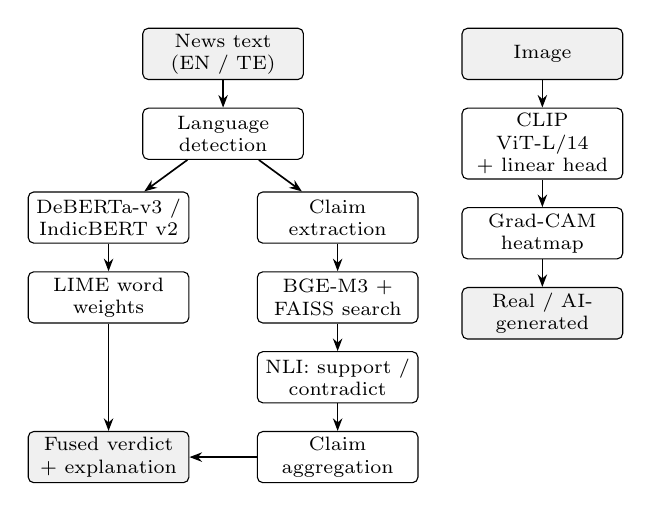
\begin{tikzpicture}[
  font=\scriptsize,
  box/.style={draw, rounded corners=2pt, align=center, minimum height=6.5mm, text width=19mm, inner sep=2pt},
  io/.style={draw, fill=gray!12, rounded corners=2pt, align=center, minimum height=6.5mm, text width=19mm, inner sep=2pt},
  arr/.style={-{Stealth[length=1.6mm]}, semithick},
  node distance=3.5mm and 3mm]
\node[io] (text) {News text\\(EN / TE)};
\node[box, below=of text] (lang) {Language\\detection};
\node[box, below left=4mm and -6mm of lang] (cls) {DeBERTa-v3 /\\IndicBERT v2};
\node[box, below=of cls] (lime) {LIME word\\weights};
\node[box, below right=4mm and -6mm of lang] (ext) {Claim\\extraction};
\node[box, below=of ext] (ret) {BGE-M3 +\\FAISS search};
\node[box, below=of ret] (nli) {NLI: support /\\contradict};
\node[box, below=of nli] (agg) {Claim\\aggregation};
\node[io] (fuse) at (lime |- agg) {Fused verdict\\+ explanation};
\node[io, right=6mm of text, xshift=14mm] (img) {Image};
\node[box, below=of img] (clip) {CLIP ViT-L/14\\+ linear head};
\node[box, below=of clip] (cam) {Grad-CAM\\heatmap};
\node[io, below=of cam] (iout) {Real / AI-\\generated};
\draw[arr] (text) -- (lang);
\draw[arr] (lang) -- (cls);
\draw[arr] (lang) -- (ext);
\draw[arr] (cls) -- (lime);
\draw[arr] (ext) -- (ret);
\draw[arr] (ret) -- (nli);
\draw[arr] (nli) -- (agg);
\draw[arr] (lime) -- (fuse);
\draw[arr] (agg) -- (fuse);
\draw[arr] (img) -- (clip);
\draw[arr] (clip) -- (cam);
\draw[arr] (cam) -- (iout);
\end{tikzpicture}
\caption{TruthLens AI architecture. The text classifier and claim verifier run on the same article and are fused; images go through a separate CLIP-based detector.}
\label{fig:arch}
\end{figure}

\subsection{Language detection and text classification}
An input is treated as Telugu when more than 30\% of its letters fall in the Telugu Unicode block (U+0C00 to U+0C7F); otherwise it is English. The user can override this choice. English text goes to DeBERTa-v3-large (435M parameters) and Telugu text to IndicBERT v2 (MLM-only checkpoint). Both are fine-tuned as binary classifiers on title plus body, truncated to 256 tokens. The classifier returns $p_{\text{fake}}$, the softmax probability of the fake class.

\subsection{Image detection}
Following Ojha et al. \cite{ojha2023universal}, we freeze the CLIP ViT-L/14 image encoder \cite{radford2021clip,dosovitskiy2021vit}, take the projected 768-dimensional embedding of each image after resizing and centre-cropping to $224\times224$, and train a single linear layer on top. Only 1,538 weights are learned, so training takes minutes once features are cached.

\subsection{Explanations}
For text, LIME \cite{ribeiro2016lime} removes random subsets of words, runs the classifier on 200 perturbed copies, and fits a weighted linear model. We split on whitespace rather than with an English tokenizer so that Telugu words are not broken into pieces. The 12 words with the largest weights are highlighted in the article, red when they push toward fake and green when they push toward real.

For images, Grad-CAM \cite{selvaraju2017gradcam} is applied to the first layer normalisation of the last ViT block. The 256 patch tokens are reshaped to a $16\times16$ grid, weighted by the gradient of the predicted class, upsampled and overlaid on the image.

\subsection{Contradiction-aware claim verification}
\label{sec:verify}

\textit{Claim extraction.} English text is split into sentences with spaCy; Telugu text is split on sentence punctuation. Questions, sentences under five words (three for Telugu) or over 80 words, and sentences that start with opinion markers such as ``I think'' or ``share this'' are dropped. Each remaining sentence $s$ gets a check-worthiness score
\begin{equation}
\begin{split}
w(s) = 1 &+ 0.8\,\min(e_s,3) + \mathbf{1}[\text{number}]\\
&+ 0.3\,\min(c_s,4) + 0.7\,\mathbf{1}[\text{fact verb}],
\end{split}
\end{equation}
where $e_s$ is the number of named entities and $c_s$ the number of capitalised words. The capitalisation and verb terms apply to English only. The eight highest-scoring sentences, in article order, are the claims.

\textit{Evidence retrieval.} Evidence passages are stored as JSON lines and embedded with BGE-M3 \cite{chen2024bgem3}, which handles English and Telugu in one vector space. A FAISS inner-product index \cite{johnson2021faiss} over normalised vectors returns the top $k=3$ passages by cosine similarity, and passages below 0.45 are discarded. When an API key is set, results from the Google Fact Check Tools API are added.

\textit{Verdict per claim.} For claim $c$ with evidence set $E_c$, an NLI model scores each pair (evidence as premise, claim as hypothesis). English uses DeBERTa-v3-large trained on MNLI, FEVER-NLI, ANLI, LingNLI and WANLI \cite{laurer2024nli}; Telugu uses multilingual mDeBERTa-v3-base. Let
\begin{equation}
s^{+}_c = \max_{e\in E_c} p_{\text{ent}}(e,c), \qquad s^{-}_c = \max_{e\in E_c} p_{\text{con}}(e,c).
\end{equation}
With threshold $\tau = 0.5$, the label is
\begin{equation}
y_c = \begin{cases}
\text{Contradiction}, & s^{-}_c \ge \tau \text{ and } s^{-}_c \ge s^{+}_c,\\
\text{Support}, & s^{+}_c \ge \tau,\\
\text{Unknown}, & \text{otherwise,}
\end{cases}
\end{equation}
with confidence $s^{-}_c$, $s^{+}_c$, or $1-\max(s^{+}_c,s^{-}_c)$ respectively. Contradiction is tested first. A single passage that clearly refutes a claim outweighs passages that only partly agree, which is how a human fact-checker treats a refutation. If $E_c$ is empty the claim is Unknown.

\textit{Aggregation and fusion.} With $n$ claims and confidences $q_c$, the article score is
\begin{equation}
S = \frac{1}{n}\sum_{c} \begin{cases} q_c & y_c=\text{Support}\\ -q_c & y_c=\text{Contradiction}\\ 0 & y_c=\text{Unknown}\end{cases},
\qquad C = \frac{S+1}{2},
\end{equation}
so $C\in[0,1]$ is a credibility score. The article is ``Unverified'' if no claim is supported or contradicted, ``Likely Misleading'' if $S\le-0.2$, ``Likely Credible'' if $S\ge0.2$, and ``Mixed Evidence'' otherwise. When the article is not Unverified, the final fake risk averages the two sources,
\begin{equation}
r = \tfrac{1}{2}\left(p_{\text{fake}} + (1-C)\right),
\end{equation}
and the article is labelled Fake when $r\ge0.5$. If only one source is available, $r$ is that source alone. A user therefore always sees which source decided the verdict.

\section{Implementation}

The backend is a FastAPI service with endpoints for text, image, claim and batch checks; models load on first use and are cached, and every check is stored in SQLite for the history page. The frontend is a React and Vite single-page application. Batch mode accepts a CSV file with a text column or a ZIP of images and returns a downloadable CSV of results. A Python launcher creates the virtual environment, installs dependencies, starts both servers and opens the browser, so the system runs on Windows, Linux or macOS with one command.

Training ran on a single NVIDIA T4 (16 GB) in a free cloud notebook. Table~\ref{tab:hyper} lists the settings. Text models use AdamW with 10\% linear warm-up, weight decay 0.01, mixed precision, and early stopping with patience 2 on validation F1.

\begin{table}[t]
\caption{Training settings}
\label{tab:hyper}
\centering
\footnotesize
\begin{tabular}{@{}lcccc@{}}
\toprule
Model & LR & Batch$^{a}$ & Epochs & Max len \\
\midrule
DeBERTa-v3-large & $1\times10^{-5}$ & 32 & 2 & 256 \\
BERT-base (baseline) & $2\times10^{-5}$ & 32 & 3 & 256 \\
IndicBERT v2 & $3\times10^{-5}$ & 32 & 4 & 256 \\
CLIP linear head & $1\times10^{-3}$ & 64 & 30 & 224 px \\
\bottomrule
\multicolumn{5}{@{}l}{\scriptsize $^{a}$Effective batch after gradient accumulation.}
\end{tabular}
\end{table}

\section{Results}

\subsection{Classification}
Table~\ref{tab:cls} gives test-set results for the three trained classifiers and the BERT baseline.

\begin{table}[t]
\caption{Classification results on held-out test sets (fake or AI-generated is the positive class; TF-IDF rows use the bias-check split)}
\label{tab:cls}
\centering
\footnotesize
\setlength{\tabcolsep}{3.2pt}
\begin{tabular}{@{}lccccc@{}}
\toprule
Model & Acc. & Prec. & Rec. & F1 & AUC \\
\midrule
TF-IDF + LR (EN) & 0.962 & -- & -- & 0.957 & -- \\
BERT-base (EN) & 0.9884 & 0.9901 & 0.9844 & 0.9872 & 0.9993 \\
DeBERTa-v3-L (EN) & \textbf{0.9972} & \textbf{0.9979} & \textbf{0.9960} & \textbf{0.9970} & \textbf{0.9999} \\
\midrule
TF-IDF + LR (TE) & 0.871 & -- & -- & 0.875 & -- \\
IndicBERT v2 (TE) & 0.9305 & 0.9104 & 0.9550 & 0.9322 & 0.9832 \\
\midrule
CLIP ViT-L/14 (img) & 0.9371 & 0.9367 & 0.9376 & 0.9371 & 0.9839 \\
\bottomrule
\end{tabular}
\end{table}

On the 12,727 English test articles, BERT-base makes about 148 errors and DeBERTa-v3-large about 36, so the larger model removes three quarters of the baseline's mistakes. Measured against the TF-IDF model the picture is less flattering: the bag-of-words model already reaches 96.2\%, so DeBERTa's gain over a model with no grasp of language is 3.5 points. We read this as evidence that most of WELFake can be separated by vocabulary, and that the remaining few percent is where the transformer earns its cost.

The Telugu model reaches 93.1\%, six points below English. Three differences explain most of the gap: it trains on 7,200 articles instead of 18,000, each article is cut to 120 words before translation, and machine translation adds noise to both classes. Its gain over the Telugu TF-IDF model is 6.0 points, larger than in English, which suggests the classifier relies less on surface vocabulary when that vocabulary is noisier. Its errors lean one way: fake recall is 95.5\% and real recall 90.6\%, so it flags some real articles as fake more often than it misses fake ones. For a tool that asks readers to check before forwarding, that is the safer direction to err.

The image detector reaches 93.7\% with ROC-AUC 0.984, and its errors are balanced (real recall 93.7\%, AI-generated recall 93.8\%). Only the 768 by 2 linear head is trained, on 40,000 of CIFAKE's 100,000 training images.

\subsection{Claim verification}
\label{sec:claimres}
Table~\ref{tab:claims} compares our decision rule with a similarity-only baseline that labels a claim Support whenever a passage with cosine similarity of at least 0.45 exists, and Unknown otherwise. This is what a retrieval system without NLI can offer. For FEVER and Climate-FEVER the gold evidence sentences are given, so the table measures the verdict stage alone; the curated set runs the full pipeline, retrieval included, over the system's own evidence corpus.

\begin{table}[t]
\caption{Claim verification (macro-F1 over Support, Contradiction, Unknown)}
\label{tab:claims}
\centering
\footnotesize
\setlength{\tabcolsep}{4pt}
\begin{tabular}{@{}llccc@{}}
\toprule
Benchmark & Method & Acc. & Macro-F1 & F1 Contr. \\
\midrule
\multirow{2}{*}{FEVER} & Similarity only & 0.400 & 0.292 & 0.000 \\
 & TruthLens & \textbf{0.846} & \textbf{0.847} & \textbf{0.855} \\
\midrule
\multirow{2}{*}{Climate-FEVER} & Similarity only & 0.340 & 0.181 & 0.000 \\
 & TruthLens & \textbf{0.509} & \textbf{0.467} & \textbf{0.663} \\
\midrule
\multirow{2}{*}{Curated$^{a}$} & Similarity only & 0.525 & 0.487 & 0.000 \\
 & TruthLens & \textbf{1.000} & \textbf{1.000} & \textbf{1.000} \\
\bottomrule
\multicolumn{5}{@{}l}{\scriptsize $^{a}$Full pipeline: retrieval over the system's corpus, then NLI.}
\end{tabular}
\end{table}

On FEVER (300 claims per class) the decision rule labels 84.6\% of claims correctly, with F1 between 0.79 and 0.90 for every class. The similarity baseline calls almost everything Support, because refuting evidence is about the same subject as the claim and is just as similar to it; it finds none of the 300 refuted claims. This is the gap that the NLI step closes.

Climate-FEVER is much harder. Its claims were collected from the web and its evidence sentences were retrieved from Wikipedia, so a sentence is often related to the claim without settling it. TruthLens still catches 79\% of the refuted claims (119 of 150), but it labels only 15\% of the supported claims Support (precision 0.77); most of the rest come back Unknown. The NLI model asks for close entailment and real-world evidence rarely gives it. For a fact-checking aid we consider this the safer failure: a supported claim marked Unknown costs the reader a look at the evidence, while a false claim marked Supported would mislead them.

On the curated set the full pipeline, retrieval included, labels all 40 claims correctly, 30 English and 10 Telugu, while the similarity baseline again marks all 17 contradicted claims as supported. This set was written by us against our own 40-passage corpus, so it checks that retrieval, language routing and the decision rule work together; it is not a measure of accuracy on unseen claims, for which FEVER and Climate-FEVER are the better guide.

\subsection{Telugu verification}
The English NLI model was not trained on Telugu, so we measured both NLI models on 1,000 IndicXNLI Telugu test pairs \cite{aggarwal2022indicxnli}. Table~\ref{tab:te} shows the result. The English model, though larger and stronger on English, is barely above chance (33\%) on Telugu, while the multilingual model reaches 74.2\%. This is why Telugu claims are routed to mDeBERTa. The 74.2\% is also a reminder that Telugu verification is weaker than English verification in our system.

\begin{table}[t]
\caption{Three-class NLI on IndicXNLI Telugu (1,000 pairs)}
\label{tab:te}
\centering
\footnotesize
\begin{tabular}{@{}lcc@{}}
\toprule
NLI model & Accuracy & Macro-F1 \\
\midrule
DeBERTa-v3-large (English only) & 0.400 & 0.396 \\
mDeBERTa-v3-base (multilingual) & \textbf{0.742} & \textbf{0.745} \\
\bottomrule
\end{tabular}
\end{table}

\begin{figure}[t]
\centering
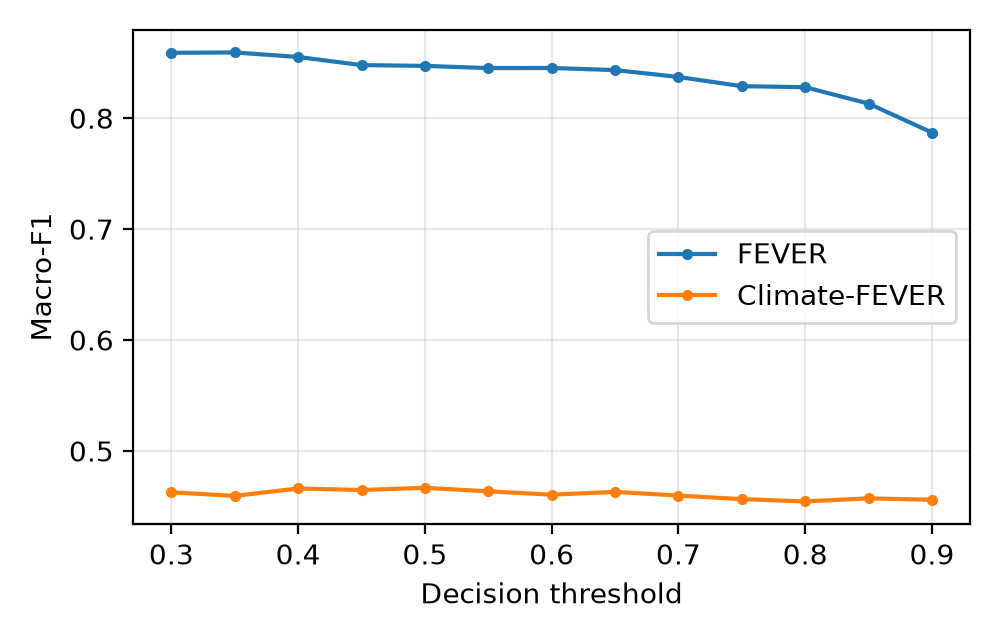
\includegraphics[width=0.92\columnwidth]{figures/threshold_sweep.png}
\caption{Macro-F1 of the decision rule as the threshold $\tau$ changes.}
\label{fig:sweep}
\end{figure}

Fig.~\ref{fig:sweep} shows how the threshold $\tau$ affects macro-F1. On FEVER the best value is 0.859 at $\tau=0.35$, slightly above the 0.847 at our default of 0.5, and the score falls to 0.787 at $\tau=0.9$ as more claims become Unknown. On Climate-FEVER the curve is flat, between 0.455 and 0.467, so the weak Support recall there comes from the NLI scores themselves rather than from the choice of threshold. We kept $\tau=0.5$ because it was fixed before the evaluation and a lower value would admit more weak support in the application.

\section{Discussion and Limitations}

The clearest limitation is the evidence corpus. The system can only contradict a claim if a passage about that claim is in the index, and the bundled corpus has 40 hand-checked passages on Indian current affairs, science and common health hoaxes. Claims outside it come back Unknown. The corpus is a folder of JSON-lines files and a helper script adds Wikipedia articles, but a deployed system would need a much larger and regularly updated index or the fact-check API.

The Telugu classifier is trained on translated English news. Its articles are about United States politics, translated into Telugu, so it has not seen the topics, names and phrasing of local Telugu misinformation. A native Telugu dataset with labels that do not follow writing style would be the most useful next step.

CIFAKE images are $32\times32$ CIFAR-style pictures from a single generator. A detector trained on them is not evidence of performance on full-resolution images from current generators, and we present the image result as a proof of concept.

Finally, the WELFake bias check shows that high accuracy on that dataset does not by itself demonstrate an understanding of truthfulness. This is one reason we added claim verification: its output can be checked against named sources, while a classifier's output can only be trusted or not.

\section{Conclusion}

TruthLens AI checks English and Telugu news and images in one interface, explains each verdict, and, for text, reports which individual claims are supported or contradicted by evidence. On benchmarks with gold evidence, the contradiction-aware rule separates refuted claims from supported ones, which a similarity-only method cannot do. Future work is a native Telugu dataset, a larger multilingual evidence index, and image training on high-resolution output from current diffusion models.

\bibliographystyle{IEEEtran}
\bibliography{refs}

\end{document}
